%%%%%%%%%%%%%%%%%%%%%%%%%%%%%%%%%%%%%%%%%%%%%%%%%%%%%%%%%%%%
\documentclass[a4paper,english]{report}    % list options between brackets

\RequirePackage{color}
%\RequirePackage{float}
\RequirePackage{amsfonts}
\RequirePackage{amsmath}
%\RequirePackage{alltt}
%\RequirePackage{ae}
\RequirePackage{times}
\RequirePackage{fancyhdr}
\RequirePackage{graphicx} 
\RequirePackage{verbatim} 
\RequirePackage{makeidx}
\RequirePackage{hyperref}

\hypersetup{
    bookmarks=true,         % show bookmarks bar?
    unicode=false,          % non-Latin characters in Acrobat�s bookmarks
    pdftoolbar=true,        % show Acrobat�s toolbar?
    pdfmenubar=true,        % show Acrobat�s menu?
    pdffitwindow=false,     % window fit to page when opened
    pdfstartview={FitH},    % fits the width of the page to the window
    pdftitle={ElmerGrid Manual},    % title
    pdfauthor={Peter Råback, CSC - IT Center for Science},     % author
%    pdfsubject={Subject},   % subject of the document
%    pdfcreator={Creator},   % creator of the document
%    pdfproducer={Producer}, % producer of the document
%    pdfkeywords={keywords}, % list of keywords
    pdfnewwindow=true,      % links in new window
    colorlinks=true,       % false: boxed links; true: colored links
    linkcolor=black,          % color of internal links
    citecolor=black,        % color of links to bibliography
    filecolor=black,      % color of file links
    urlcolor=black           % color of external links
}



\makeindex             

%%%%%%%%%%%%%%%%%%%%%%%%%%%%%%%%%%%%%%%%%%%%%%%%%%%%%%%%%%%%

% Use these to make the printable area bigger
% Also have the option 'ownsize' active in the documentclass
\setlength{\hoffset}{-15mm}
\setlength{\voffset}{-10mm}
\addtolength{\textwidth}{30mm}
\addtolength{\textheight}{20mm}
%\addtolength{\headwidth}{30mm}


% Command file syntax stuff
\definecolor{SifCol}{rgb}{0.5,0.5,0.5}
%\definecolor{SifCol}{rgb}{1,1,1}

% Index for keywords
\newcommand{\sifitem}[2]{\item[\tt{#1}]\index{#1}\hspace{1mm}{\color{SifCol}\hspace{1mm}\tt{#2}}\newline} 
%item with two fields but no text
\newcommand{\sifitemnt}[2]{\item[\tt{#1}]\index{#1}\hspace{1mm}{\color{SifCol}\hspace{1mm}\tt{#2}}} 


\newcommand{\sifbegin}{\begin{description}}
\newcommand{\sifend}{\end{description}}
\newcommand{\modinfo}[2]{{\bf{#1}}: {#2}\newline}

\newcommand{\ttbegin}{\begin{alltt}}
\newcommand{\ttend}{\end{alltt}}
\newcommand{\ttitem}[1]{\item[\tt{#1}]\mbox{}\\}
\newcommand{\keno}{$\backslash$}


\newcommand{\Sf}[1]{\textsf{#1}}
\newcommand{\Bf}[1]{{\sffamily\bfseries}}

\newcommand{\URL}[1]{\texttt{#1}}

% Some new commands...
\def\xwin{X Window System}
\def\xbr{Xbrowse}
\def\prag{\Tt{\#pragma}}

\newcommand{\inxgra}[2]{{\centerline{\includegraphics[width=#1]{#2}}}}
\newcommand{\inygra}[2]{{\centerline{\includegraphics[height=#1]{#2}}}}
\newcommand{\incgra}[2]{{\centerline{\includegraphics[height=#1]{#2}}}}

\providecommand{\ftn}{Fort\-ran~90}
\providecommand{\Idx}[1]{{#1}\index{#1}}


%%%%%%%%%%%%%%%% Math definitions for Elmer Solver Manuals %%%%%%%%%%%%%%%%%
\newcommand{\Bfm}[1]{\mbox{\boldmath{${#1}$}}}

\newcommand{\tensorspace}[1]{\boldsymbol{#1}}         % Sets of tensors are bold italic
\newcommand{\tensor}[1]{\boldsymbol{#1}}              % Tensors are bold italic
\newcommand{\point}[1]{\mathbf{#1}}                   % Points are bold upright
\newcommand{\pointf}[1]{\mathbf{#1}}                  % Point-valued functions are bold upright
\newcommand{\pointfm}[1]{\mbox{\boldmath{${#1}$}}}    % Point-valued functions for math symbols

\DeclareMathOperator{\grad}{\mathbf{grad}}            % The spatial gradient operator
\newcommand{\Grad}{\mbox{\boldmath{${\nabla}$}}}      % gradient with respect to the points of the reference configuration
\DeclareMathOperator{\curl}{\mathbf{curl}}            % The spatial curl operator
\DeclareMathOperator{\Curl}{\mathbf{Curl}}            % curl with respect to the points of the reference configuration
\DeclareMathOperator{\rot}{\mathbf{rot}}              % rot operator defined for scalars
\DeclareMathOperator{\divs}{\mathrm{div}}             % scalar-valued divergence
\DeclareMathOperator{\divvec}{\mathbf{div}}           % vector-valued divergence
\DeclareMathOperator{\Divvec}{\mathbf{Div}}           % vector-valued divergence w. r. t. the points of the reference configuration
\newcommand{\Div}{\nabla\cdot}                        

%\newcommand{\Vec}[1]{\vec{#1}}
%\newcommand{\Vec}[1]{\mathify{\mathbf{#1}}}

%\newcommand{\Matr}[1]{\mbox{${#1}$}}                  % Matrices are just italic to differentiate between true tensors and matrices
\newcommand{\Matr}[1]{{#1}}                     % Matrices
\newcommand{\Der}[2]{\frac{\partial{#1}}{\partial{#2}}}
\newcommand{\Secder}[2]{\frac{\partial^2{#1}}{\partial{#2}^2}}
\newcommand{\Inv}[1] {\frac{1}{#1}}


% Make the headings fancier
\pagestyle{fancy}

\lhead[\normalfont\small\bf\thepage]{\normalfont\small\slshape\rightmark}
\rhead[\small\slshape\lefthead]{\normalfont\small\bf \thepage}
%\setlength{\headrulewidth}{0.4pt}
%\renewcommand{\chaptermark}[1]{\markright{\bf \chaptername \ \thechapter.\ #1}{}}
%\renewcommand{\chaptermark}[1]{\markright{\bf \thechapter.\ #1}{}}
\renewcommand{\sectionmark}[1]{}
\renewcommand{\subsectionmark}[1]{}
\cfoot{}

% This sets the Elmer version in the documentation
%\newcommand{\elmerversion}{6.0}



% This sets the Elmer version in the documentation
\newcommand{\elmerversion}{8.4}


%%%%%%%%%%%%%%%%%%%%%%%%%%%%%%%%%%%%%%%%%%%%%%%%%%%%%%%%%%%%

\title{\Huge{\bf ElmerGrid Manual}}
\author{Peter R{\aa}back \\ \\ CSC -- IT Center for Science}
\date{28 Aug 2020}

%%%%%%%%%%%%%%%%%%%%%%%%%%%%%%%%%%%%%%%%%%%%%%%%%%%%%%%%%%%%

\begin{document}
\maketitle

\chapter*{Get Started with Elmer}

\section*{About this document}

This document, Get Started with Elmer, is intended to help anyone who has just downloaded Elmer and would like some help getting started.\\

The first three chapters are provided specifically for Windows users, with detailed instructions to download, install, and start using Elmer.  The instructions have been tested on Windows 10.\\

The rest of the chapters in this document generally apply to all users, running Windows, Linux, and MacOS.\\

Topics discussed include:

\begin{itemize}
  \item Paraview and ElmerVTK for post processing Elmer results
  \item Using Elmer, where to find test cases, tutorials, the Elmer user forum, and youtube video
  \item Parallel operation of Elmer
  \item External tools with Elmer, such as Gmsh and Salome, providing examples of creating multiple bodies
  \item Elmerfem Wiki, a copy of the old wiki
  \item Installing the Elmer Virtual Machine
  \item Installing Elmer in Linux
\end{itemize}


The present manual corresponds to Elmer software version~\elmerversion{}.\\

Latest documentations and program versions of Elmer are available (or links are provided) at \url{http://www.csc.fi/elmer}. \\

\section*{Copyright information}

This document is licensed under the Creative Commons Attribution-NonCommerical 3.0 License.  To view a copy of this license, visit \url{http://creativecommons.org/licenses/by-nc/3.0/}.\\

Initially this document, Get Started with Elmer, has been written by Rich Bayless.  External contributions are welcome.





%%%%%%%%%%%%%%%%%%%%%%%%%%%%%%%%%%%%%%%%%%%%%%%%%%%%%%%%%%%%

% Table of contents:
\setcounter{secnumdepth}{2}
\setcounter{tocdepth}{1}  % set this to 1 in the final version

\phantomsection
\addcontentsline{toc}{chapter}{Table of Contents}
\tableofcontents

%%%%%%%%%%%%%%%%%%%%%%%%%%%%%%%%%%%%%%%%%%%%%%%%%%%%%%%%%%%%

\newpage

% change the plain style used for chapter pages
\fancypagestyle{plain}{
\lhead{}
\rhead{}
\rfoot{
\includegraphics[width=18mm]{by-nd}}
\lfoot{\footnotesize{CSC -- IT Center for Science}}
\chead{}
%\cfoot{\bfseries \thepage}
\cfoot{}
\renewcommand{\headrulewidth}{0.0pt}
}

% and the fancy style used elsewhere
\pagestyle{fancy}
\rhead{\bfseries \thepage}
\lhead{\bfseries \rightmark}
\rfoot{
\includegraphics[width=18mm]{by-nd}}
\lfoot{\footnotesize{CSC -- IT Center for Science}}
\chead{}
\cfoot{}
\renewcommand{\headrulewidth}{0.4pt}
\renewcommand{\footrulewidth}{0.4pt}



%%%%%%%%%%%%%%%%%%%%%%%%%%%%%%%%%%%%%%%%%%%%%%%%%%%%%%%%%%%%

\graphicspath{{./}{figures/}}
\chapter{Overview of ElmerGrid}

\section{Introduction}

ElmerGrid is a simple mesh generator and 
mesh manipulation utility. 
It is an appropriate tool for generating structured meshes for 
simple 1D, 2D, and 3D geometries. 
It can also read meshes generated by other mesh generators and 
manipulate them. Among the possible operations are
scaling, changing of element type, 
defining boundaries, or partitioning the mesh for parallel solution, 
for example.

ElmerGrid was originally a side product of research done in the area
of silicon carbide crystal growth.
The main goal was to write a simple mesh generator for multiphysical
problems where different meshes based on the same geometry were needed for different physical problems.
Since that the software has been modified to meet the 
needs of Elmer development.
Thus the name has been changed from Quickmesh to ElmerGrid.
Because ElmerGrid was never designed to be a stand-alone mesh generator 
it has been developed in an uncontrolled manner. The data structures 
are not optimal for all the added features. Therefore the software may
at times cause problems.

This chapter shortly describes the main 
capabilities of the program.


\section{Usage}
The executable binary of the program is named {\tt ElmerGrid}.
It may be started with no arguments at
all. Then the following help text is automatically 
displayed.

\verbatiminput{ElmerGrid.info}

As may be seen the user may choose between several 
input and output formats. The format is specified 
by an integer number (or an appropriate string) and the file name that is given may 
or may not have the appropriate suffix.


\section{Input formats}

The ElmerGrid code has two different operation modes.
In the one all the information is read from a command file.
Alternatively all necessary data may be read from 
from the inline arguments. 

The native formats of the code are thus the command file 
with the suffix \texttt{.eg} and the 
native geometry format that has the suffix \texttt{.grd}. 
Note that most commands that may be given in the command file 
may also be given in the geometry format. 

Additionally there are several other input formats
that helps in linking the Elmer software with other pre- and 
postprocessors. 
The other formats may
not always be used to create a complete
model with boundary conditions. Also their functionality 
does not include all the possible commands.

\begin{description}
\item \texttt{1)  .grd      : ElmerGrid file format} \\
The native ElmerGrid format is  described in a separate section.

\item \texttt{2)  .mesh.*  : Elmer output format} \\
Input format for ElmerSolver consisting of separate header,
node, coordinate and topology files.

\item \texttt{3)  .ep      : Elmer input format} \\
This format is the same that
ElmerSolver uses in saving the results to be 
postprosessed with ElmerPost. 

\item \texttt{4)  .ansys    : Ansys input format} \\
This format is the input format 
created by the preprosessor of Ansys using a special
Ansys macro.
An example is given in later chapters.

\item \texttt{5)  .inp    : Abaqus input format by Ideas} \\
This format is the input format 
created by Ideas preprocessor for Abaqus.

\item \texttt{6)  .fil    : Abaqus output format} \\
This format is the output format 
created by the solver of Abaqus.

\item \texttt{7)  .FDNEUT  : Fidap neutral file} \\
Also created by Gambit, the preprocessor of Fluent.

\item \texttt{8) .unv : Universal mesh file format} \\
A subset of the universal mesh file format commands may be read by ElmerGrid.

\item \texttt{9)  .mphtxt   : Comsol mesh format} \\
The mphtxt format created by Comsol Multiphysics. 

\item \texttt{10)  .dat      : Fieldview format} \\
This may be used with Gridgen preprocessor.

\item \texttt{11) .node,.ele: Triangle 2D mesh format} \\
Read in meshes created by Triangle 2D Delaunay mesh generator.

\item \texttt{12) .mesh     : Medit mesh format} \\
Format of Medit mesh generation program.

\item \texttt{13) .msh      : GID mesh format} \\
Format of GID mesh generation program.

\item \texttt{14) .msh      : Gmsh mesh format} \\
Format of Gmsh mesh generation program.

\item \texttt{15) .ep.i     : Partitioned ElmerPost format} \\
Partitioned Elmer results created by parallel computing. 

\item \texttt{16) .2dm      : FVCOM mesh format} \\
2D triangular format for the Unstructured Grid Vinite Volume Community Ocean Model, FVCOM.
  
\end{description}

\section{Output formats}
The supported output formats are all different 
formats of Elmer software. Additionally, there are some undocumented formats.
Thus, if you need to export some data from Elmer format you may
ask for the possibilities. 


\begin{description}

\item \texttt{1)  .grd     : ElmerGrid file format} \\
The native format, may be used to refresh the input file if it becomes
corrupted or outdated.

\item \texttt{2)  .mesh.*   : ElmerSolver file format} \\
Format that may be used in Elmer calculations.
In a single-processor version 
the input is divided to four different files with 
suffixes, \texttt{mesh.boundary}, \texttt{mesh.elements},
\texttt{mesh.header} and \texttt{mesh.nodes}.

The command-line parameters \texttt{-part} and \texttt{-metis} 
activate the partitioned 
input format for the ElmerSolver. 
The ending is \texttt{.part.*} and the 
files are saved to 
subdirectory with suffix \texttt{.part.n}, where
\texttt{n} is the running number of the partition.

\item \texttt{3)  .ep       : ElmerPost file format} \\
Format for Elmer postprosessing. This is particularly handy for tuning the
mesh before it is used in the solution. Then the only variable that is saved is 
the node index referred to by field variable \texttt{Number}.

\item \texttt{4)  .msh      : Gmsh file format} \\
Format for Gmsh mesh generator. This may be useful if one wants to use Gmsh to view entity numbers or mesh quality. 
Also one could use Gmsh as a tool to export meshes from Elmer project to a more commonly used format for interoperability with other software.

\item \texttt{5)  .vtu      : XML based unstructured VTK format} \\
This format may be read by software utilizing the VTK library such as Paraview. 
The format could be useful for studying the mesh prior to actual solution.



\end{description}



\section{ElmerGrid command-line arguments}

ElmerGrid has a lot of simple functionalities that may be activated 
with the right command-line arguments. Most of them may operate on
all meshes, some are limited to 2D meshes, for example. 

In the command-line operation mode
there are only three mandatory arguments: The input format,
the output format, and the name of the input file.  For example, 
to read an ElmerGrid file named \texttt{angle.grd}, and to output the
ElmerSolver files to a folder named \texttt{angle}:\\

\texttt{elmergrid 1 2 angle}\\

All other arguments are optional.

\sifbegin
\sifitem{-out}{String}
Gives an alternative name for the output file or directory. 
The default name is the same as the name of the input file
attached with an appropriate suffix. 
%
\sifitem{-in}{String}
Sometimes there are may be more than one input mesh. 
Then the name of the secondary input file may be given 
after this keyword.
%
\sifitem{-decimals}{Integer}
The number of decimals for Elmer mesh is by default set to 6.
Sometimes more decimals may be needed and this command may then
be used. This could be the case, for example, if the elements are 
small compared to the absolute values of the coordinates.
The size of the ascii file is affected by the number of 
decimals and therefore the default is quite small.
%
\sifitem{-relh}{Real}
Gives a relative density of the mesh. Value of one will have no effect
while smaller values will result to a denser mesh. This is an easy way to 
increase mesh density of ElmerGrid meshing without having to edit the .grd file. 
%
\sifitem{-triangles}{}
The meshes consisting of rectangles may be divided into 
triangles. This operation may be performed on all 2D meshes, 
not only to the ones created using ElmerGrid format.
%
\sifitem{-merge}{Real}
Sometimes when creating the computational mesh the 
different domains are not properly joined. Then it is possible to 
use this option, where nodes that are close to each other are
fused. The value given for the node separation should be smaller than
the smallest element size. Otherwise there is a risk of ruining the mesh.

For optimal computational efficiency the merging of nodes is done 
in two stages. In the first stage the nodes are ordered and in the second
stage the nodes close to each other are checked for distance. 
If distance is smaller than the critical one, then the nodes are given one
common coordinate and the other node is eliminated from the whole mesh.
%
\sifitem{-order}{Real[DIM]} 
The nodes may be ordered if the original ordering is uneconomical.
The three components gives the direction in which the nodes are reordered.
More accurately, the nodes are ordered using the 
dot product $\vec{c}\cdot\vec{r}$ as a measure.
%
The reordering of the degrees of freedom is usually performed 
within ElmerSolver and therefore 
it is usually not necessary to renumber the nodes within ElmerGrid.
%
\sifitem{-centralize}{}
Sets the center of the mesh to origin. The bounding box is used to define the size of the mesh. 
%
%\sifitem{-autoorder}{}
%This uses heuristic ordering methods to optimize the bandwidth. The same
%optimization method is used consecutively and the best choice is kept. 
%This seems, however, usually be inferior to the algorithm in 
%ElmerSolver.
%
\sifitem{-scale}{Real[DIM]}
This simply scales the coordinates of the mesh by 
multiplying with the given constants, i.e.
$x:=c_x x$, $y:=c_y y$ and $z:=c_z z$.
This is useful, for example, if the mesh is in other units that is 
preferable. 
%
\sifitem{-translate}{Real[DIM]} 
This option translates the mesh with a given vector by
simply adding the given values to the original coordinates,
i.e. $\vec{r} := \vec{r} + \vec{r}_0$.
%
\sifitem{-rotate}{Real[3]} 
The mesh may be rotated around the main axis. 
The rotation is done consecutively in all three angles.
This feature may be handy in the debugging of some equation --
in Cartesian grids the solution should be rotation invariant.
%
\sifitem{-clone}{Integer[DIM]}
The mesh may be copied so that the same 
structure is repeated over and over. The number of copies in 
each coordinate direction may be given independently.
The total number of individual copies is their product.
%
\sifitem{-clonesize}{Real[DIM]} 
By default the copies of the mesh are performed so that the 
new meshes are set directly besides the old ones. This flag may be used to define
a larger size for the mesh which enables empty space being left 
between the meshes.
%
\sifitem{-mirror}{Integer[DIM]} 
The mesh may be mirrored over the main axis. The arguments 
tell over which axis the mesh should be mirrored. If all three axis
are active then the original mesh will be eight times the size of the original one.
Note that the origin is assumed to be at zero in all directions.
%
\sifitem{-unite}{}
This option unites the ElmerGrid meshes. In every other format its currently
not possible to create more than one mesh at a time.
\sifitem{-unitenooverlap}{}
As the previous one except avoids overlapping entity numbering.
New numbers will be generated in order to avoid conflicts.
%
\sifitem{-polar}{Real}
This option maps the 2D mesh an a cylindrical shell with the radius
given as a parameter.
%
\sifitem{-cylinder}{}
This option assumes that the original 3D mesh was given in 
cylindrical coordinates $(r,\theta,z)$ and maps them to Cartesian 
coordinates $(x,y,z)$.
%
\sifitem{-reduce}{int[2]} 
This feature reduces the element order of materials at the interval
defined by the two parameters. It may be used to lower the element order 
only in parts of the geometry. For example, in fluid-structure-interaction the 
fluid could be modelled with linear elements while the 
structure might need second order elements.
%
\sifitem{-increase}{} 
Increase the element order in all the elements from one to two.
This may be used to improve computational accuracy of existing 
linear meshes by making them quadratic.
%
\sifitem{-bcoffset}{Integer}
Adds on offset to the boundary condition numbering. This may be useful for multimesh
computations where it is advisable that the same boundary numbers are not defined in 
different meshes. 
%
\sifitem{-discont}{Integer}
Sometimes the field variables behave discontinuously over a short distance.
For example, in solving the heat equation there may be a small gap between
different bodies. To account for such discontinuities the mesh should
have duplicate nodes over the discontinuity. This feature does exactly that
and saves the boundary conditions for both sides.
%
\sifitem{-connect}{Integer}
Makes the boundary to have internal connections between among its elements. This
will enable connections in the resulting finite element matrices. The feature could 
be used in setting constraints in the finite element solution. 
%
\sifitem{-removelowdim}{}
Removes boundary elements that are two or more dimensions lower than the 
highest dimensional bulk elements. 
%
\sifitem{-removeunused}{}
Removes unused nodes from the mesh. In some mesh formats there are control nodes 
that may cause problems to ElmerSolver if these are not treated.
%
\sifitem{-bulkorder}{}
Renumbers the body indexes so that every number is used. This feature may be handy 
particularly when importing meshes that have a very wild numbering of bodies.
%
\sifitem{-boundorder}{}
Renumbers the boundary element types so that every number is used. This feature may be handy 
particularly when importing meshes that have a very wild numbering of boundary elements types.
%
\sifitem{-autoclean}{}
This flag activates several of the above procedures that simplifies the mesh
for solution purposes. The lower dimensional boundary elements are removed, 
and the body and boundary element types are renumbered.
%
\sifitem{-bulkbound}{Integer[3]}
Sometimes the geometry does not include all the necessary boundary conditions. 
Then this inline parameter may be used to define a new boundary 
(first parameter) on the interval of the two given materials.
%
\sifitem{-boundbound}{Integer[3]}
Sometimes the geometry does not include all the necessary boundary conditions. 
Then this inline parameter may be used to define a new boundary 
(first parameter) on the interval of two already existing boundaries.
This makes it possible to define lines or even single points 
in 3D geometry that has only surfaces defined.
%
\sifitem{-bulktype}{Integer[3]} 
Sometimes there is a multitude of bodies that may be united with this option.
It may be easier to perform the further analysis if the number of bodies 
is not too large.
For example, in ElmerPost and ElmerGUI a very lengthy list of bodies or 
boundaries is difficult to visualize. 
%
\sifitem{-boundtype}{Integer[3]}
This option does exactly the same as the above but now for the boundary
 elements.
Again the advantage may be that the command-file will be more economical as 
if the number of boundaries is reduced.
%
\sifitem{-layer}{Integer[2] Real[2]} 
This option may be used to create boundary layers on an existing 2D mesh.
The given boundary is extruded with the given number of layers. Also the total
thickness of the layer and the desired ratio between first and last element
is given.
%
\sifitem{-layermove}{int}
This option activates a filter that is used to map the node coordinates 
so that the boundary layers are fitted within the original geometry.
%
\sifitem{-divlayer}{Integer[2] Real[2]} 
This option may be used to create boundary layers on an existing 2D mesh.
The layer is created by splitting the triangles or quadrilaterals 
along the boundary to give a structured boundary layer mesh.
%
\sifitem{-3d / -2d / -1d}{}
This option is usually not needed as the files most often have the information
of the space dimension. The exception is the creation of an example file.
3D is the default, thus the \texttt{-2d} should be used if one wants to create
a 2D example file. Also some command-line parameter lists are by default assumed to have 
three values if 2D dimension is not given.
%
\sifitem{-isoparam}{}
In creating mapped meshes by ElmerGrid the higher-order nodes may sometimes be 
oddly displaced. This utility sets the intermediate nodes to lie on the connecting lines
between the corner nodes. 
%
\sifitem{-nobound}{}
Disable the saving of boundary elements.
This may sometimes be useful if there are a lot of boundaries and one is just interested 
in the bulk elements.
%
\sifitem{-nosave}{}
Do not save anything, just do the preceding parts.
%
\sifitem{-nooverwrite}{}
If the mesh already exists don't overwrite it. This may be handy for automated
processes where we don't want to redo steps.
%
\sifitem{-timer}{}
Show the elapsed time of the ElmerGrid execution.
%
\sifitem{-infofile}{string}
File for saving information about execution times and mesh size.
\sifend
%

There are a number of inline parameters that are related only to the parallel Elmer computations.
%
\sifbegin
\sifitem{-partition}{Integer[DIM]} 
There are two methods to partition geometry for parallel computing. This
method takes each coordinate direction and divides the mesh in the number
of slices given in the parameter list. For example option
\texttt{-part 2 3 5} would split the mesh into $2\times 3 \times 5 = 30$ partitions. 
Each split is done so that the number of elements in each partition
is almost equal. The method is best suited for simple geometries 
where more generic strategies usually do not work as well.

%The last flag is an optional flag which defines additional strategies for doing the partitioing. 
%For value 0 a recursive partitioning is applied so that the partition is first done for elements and
%thereafter for nodes. For value 1 the same algorithm is applied but now first for the nodes and then for
%elements. 

%For value 2 of the optional parameter the geometry is assumed to consist of evenly distributed cells and the elements 
%are divided into each cell. Not all cells need to be active. This kind of partitioning could be ideal for evenly distributed meshes
%that follow the cell boundaries. For example, the canonical L-shaped domain is ideally partitioning by this flag.

%The value 3 for the optional parameter invokes tailored partitioning for cylindircally symmetric structures for which the division is performed 
%in $(r,\phi,z)$ coordinates rather than $(x,y,z)$. 
%
\sifitem{-partorder}{Real[DIM]} 
The simple partitioning is done by dividing the elements
into subgroups. The division is done by first ordering the nodes. This
keyword is followed by the normal vector of the desired ordering.
%
\sifitem{-parttol}{Real}
Sometimes when using the geometric partitioning we use the ideal
structured form of the mesh in the process. For example extruded meshes
may result to partitions that could not have been extruded. The remedy
is to let the elements be in the same partition if they are close enough
to each other when ordered geometrically.
%
\sifitem{-metiskway}{Integer}
This utility does the partitioning utilizing the Metis library, see
\url{http://glaros.dtc.umn.edu/gkhome/views/metis}. Metis has subroutines
for basic linear elements. Also higher order elements may be partitioned
by first neglecting the higher order nodes.

The suffix \texttt{kway} refers to the \texttt{PartGraphKway} routine of Metis. 
This may be used for the nodal and dual graph. The dual graph is recommended. 
The parameter is the desired number of partitions. 

Note that this option may not be active if the code has been compiled
without the Metis library.
%
\sifitem{-metisrec}{Integer}
This is as the previous one except the suffix \texttt{rec} refers to the \texttt{PartGraphRecursive} routine of Metis. 
This may be used for the nodal and dual graph. The dual graph is recommended. 
The parameter is the desired number of partitions. 

\sifitem{-metiscontig}{}
This flag enforces that the Metis partitions are contiguous. This means that
each partition is continuous. This may be numerically favourable and
certainly needed by some algorithms. 

\sifitem{-metisseed}{Integer}
This allows the user to change the Metis seed. The purpose for this could be
to study the effect on partitioning on the parallel solution.
Some preconditioners are not fully parallel and their success may vary between
different seed values. 

\sifitem{-partdual}{}
The Metis algorithms that need a graph to work with by default use the nodal connectivity graph. As an
alternative choice the user may enforce the use of elemental connectivity graph, i.e. the dual graph. 
This may be advantageous for the continuity of the partitions. 
%
\sifitem{-halo}{}
This flag creates a halo for the partitioning. This must be provided, for example, in
discontinuous Galerkin computations where at the boundaries the gradient information 
must also be computed. The halo is created for all nearest neighbours. 

\sifitem{-halobc}{}
This flag creates a halo for the partitioning but only around the boundary conditions. 
No new neighbourhood connections are added to the shared nodes list among the pure halo nodes. 
This could be useful if halo information is needed only around the boundaries such as is the case 
for internal discontinuity creation in parallel. 

\sifitem{-haloz}{}
This flag creates a halo for only in the z-direction such that the the next and previous partition in
the z-direction is saved. The halo has been designed to work with rotating machines and to be used with 
\texttt{-partconnect} flag.

\sifitem{-halor}{}
As the previous one but creates a halo only in radial direction.

\sifitem{-halogreedy}{}
Create halo being greedy over the partition interfaces. 

\sifitem{-indirect}{}
Creates the indirect connections in the partitioning. These are connections in 
a finite element matrix that exist between two nodes but would not be apparent if
only the partition in question would be studied. These should be not needed any more
since ElmerSolver should be able to detect them on its own. 

\sifitem{-periodic}{Integer[3]} 
If the solution of the mesh is known to be periodic ElmerSolver uses
a special kind of boundary condition. Also in partitioned meshes
used in parallel computation the periodic boundaries must be known
as they require the flow of information between opposing sides.
This option finds periodic boundaries in the given directions 
given by 0/1 logical values. If periodic boundary is found it is taken into
account in saving and partitioning the mesh.
The determination of the periodic nodes only works when there is one-to-one mapping
between the nodes on the boundaries. 
%
\sifitem{-partoptim}{}
Applies aggressive optimization to node sharing. This may not pay off since the even execution
of owned nodes is not that important. And this optimization does not affect the number of total
nodes in each partition that is determined by the partitioning algorithm. 
%
\sifitem{-partnobcoptim}{}
Do not Apply optimization for the ownership of internal boundaries. There will be problems in parallel runs if an 
internal boundary with certain flux BCs does not have both parents in the same partition. Unfortunately 
enforcing both parents to be in the same partition may also be undesirable since it may destroy the initial 
good partitioning. Therefore this flag has been made optional but those that need internal BCs in parallel
runs should be aware of the problem. 
%
\sifitem{-partbw}{}
Minimize the bandwidth of partition-partition couplings. This could be advantageous for the 
communication depending on the network connecting the nodes. 
%
\sifitem{-parthypre}{}
Number the nodes continuously partitionwise. Some linear solvers, such as Hypre, need this 
property. May be obsolete since this can be taken care by ElmerSolver also. 

\sifitem{-partzbc}{}         
Partition connected boundaries separately to partitions in z-direction. Thereafter apply the main 
strategy (e.g. Metis) to the other elements. 

\sifitem{-partrbc}{}         
Partition connected boundaries separately to partitions in r-direction. Thereafter apply the main 
strategy (e.g. Metis) to the other elements. 

\sifitem{-metisbc}{}         
Partition connected BCs separately to partitions by Metis.

\sifitem{-partlayers}{}          
When using either two of the hybrid partitioning routines where boundary is partitioned first we may extend this
partitioning to several layers of bulk elements using this flag. 
\sifend


These are keywords related to ElmerPost and are more or less obsolete. 
\sifbegin
\sifitem{-partjoin}{Integer}
Gives the number of partitions in the data to be joined. This relates only to the output format 
15 where individual .ep files are joined. 

\sifitem{-saveinterval}{Integer[3]}
In conjunction with the previous work gives the index of first and last timestep, and the
timestep interval that should be used in the merging. 

\sifitem{-nobound}{}
Disable saving of boundary elements in ElmerPost format.
\sifend





\graphicspath{{./}{figures/}}


\chapter{ElmerGrid format}

The native mesh definition format of the program is the ElmerGrid
format that has the suffix \texttt{.grd}. 
If the user gives a name for the input file that doesn't exist, then
a simple geometry file is automatically created by the program.
This may then be edited by any text editor to suit the needs of the particular case.

The ElmerGrid parser is not very bright. It knows only
a handful of keywords. If the default values are 
used the corresponding commands may be neglected. 
The commands usually assume a format where 
the keyword is followed by its arguments. 
If the arguments are on the same line then an equality sign 
``='' should be used in between. 
The parser is not case sensitive and thus the keywords may be written with 
capital or small letters, or any combination of them.


\section{ElmerGrid keywords}

\sifbegin
\sifitem{Version}{210903}
Gives the version of the current input file. This should not be changed unless
the format is changed. The parser should be downward compatible also with the older
format of the input file but the new format is preferred.
%
\sifitem{MATC}{Logical}
Setting this keyword to be true activates the MATC parser. As an effect all statements 
starting with the \$ sign will be evaluted by MATC. This enables parametrisized mesh generation,
for example. For more information look at the MATC manual. Note that if this does not work the 
version of ElmerGrid may have been compiled without MATC. 
%
\sifitem{Coordinate System}{String}
The choices are Cartesian 1D, Cartesian 2D, Cartesian 3D, Polar and 
Axisymmetric. Axisymmetric and Cartesian 2D have currently
no difference.
A Cartesian 3D grid is the default.
%
\sifitem{Subcell Divisions}{Integer[DIM]} 
The mesh is composed of subcells that are 
topologically squares. 
This keywords should be followed by the 
number of subcells in the main directions,
$n_1$, $n_2$ and $n_3$.
Thus the number of 
arguments may be 1, 2 or 3 depending on the dimension of the geometry 
definition. 
\sifitem{Subcell Limits i}{Real[]}
The size of the subcells are defined by $n_i+1$ boundaries
in each coordinate direction. These values define the physical 
dimensions of the mesh before possible manipulation. 
This keyword exists for all active coordinate directions.  
%
\sifitem{Subcell Sizes i}{Real[]}
An alternative way to give the subcell sizes is to give the size of 
each subcell in each coordinate direction. 
The subcell limits are then the cumulative sum of these sizes.
%
\sifitem{Subcell Origin i}{Real[]}
When the subcells are defined by the sizes the user may also define the origin 
in each direction. The origin may be a real number or also some of the following 
strings, \texttt{Left}, \texttt{Center}, \texttt{Right}.
%
\sifitem{Material Structure}{Integer[][]}
The subcells form a $n_1 \times n_2$ matrix in 2D. 
The material structure of this plane may therefore be given by a matrix 
consisting of integers relating to different materials.
These numbers may then later be referred
when creating the mesh and boundary conditions.
In 1D the structure is simply a vector.
In 3D the material structure refers to the structure of the 
$xy$-plane before extrusion or rotation takes place. 
%
\sifitem{Materials Interval}{Integer[2]} 
Elements are created only for those materials that 
lie in the interval defined by the two integers.
This is on easy way to define different meshes for different physical
phenomena.
In 3D the interval refers to the materials that should be present
in the extrusion. 
%
\sifitem{Extruded Sructure}{}
The keyword may be used to define the layered 
structure of the geometry. Otherwise the extruded structure is just the same
as the material structure in the plane. 
The definition must include $n_3$ lines with three integers on each. 
The first two integers define the materials interval that is extruded and
the third one the new material index of the extruded layer.
Materials outside the interval are not extruded and therefore 
materials may selectively be dropped out during extrusion process. 
If the new material has value zero then the corresponding material layer in the 
extruded structure remains unaltered.
This feature may, for example, be useful in MEM-applications. 

When the 2D geometry is extruded the rectangular elements 404, 408 and 409 result to 
elementtypes are 808, 820 and 827 (using Elmer notation). 
Also linear triangles may be extruded and they result to 
linear prisms of type 606.
%
\sifitem{Extruded Material Mappings}{}
Sometimes the previous way of defining the extruded structure is not flexible enough. Then
the user may given for each extruded layer the mapping between initial and extruded material indexes.
This enables any kind of extruded structures be created. There will be $n_3$ lines and 
each line should have \texttt{MAX(material)} entries. 
%
\sifitem{Extruded BC Offset}{Integer}
When the mesh is extruded into 3D new boundaries will be created. By default the numbering of boundaries is such that 
each boundary index number is used and a heuristic method for the numbering defines the indexes. This may be difficult for the 
user since there is no way of knowing for sure what the indexes will be. This keyword enforces the new BCs on the extruded layers 
to have deterministic indexes. The first layer will get indexes $N_{offset}+N_{2D}$ the following will have an additional offset 
of $N_{offset}$ etc.  
%
\sifitem{Extruded Helicity}{Real}
When the geometry is extruded in z-direction the user may optionally give a constant skew to the mesh by 
giving the helicity of the mesh using this keyword. For example, value 360.0 means a full rotation during 
the extruded distance. 
%
\sifitem{Geometry Mappings}{}
The grid is by default rectangular since all the subcells are also
rectangular. Non-rectangular shapes may be introduced by mapping
the straight lines separating the subcells to lines represented by 
analytical functions. 
The mapping may be performed in the $xy$-plane or out of the plane.
The number of the mappings is calculated automatically and therefore 
the field should be ended by \texttt{End}.

If the mode of the mapping is more than 50 then 
the mapping is performed out of plane while mappings 
in the plane is the default.
Mapping out of the plane makes the 2D plates to become 3D shells.

This keyword activates mappings as in the case of mappings in plane 
but now the mapping is performed 
out of the plane. 
Thus the 2D geometry becomes 3D geometry.
This way some simple 3D shells may be created. 
If in addition, the coordinate system is set to be polar this 
third coordinate is treated as radius $r$ and the second
coordinate as angle $\phi$. 
%
\sifitem{Polar Radius}{Real}
If the coordinate system is chosen to be polar then 
the values defining the grid are $(z,\theta)$.
When saving the mesh these are mapped into cartesian coordinates.
There may be an offset in the radius when using the polar coordinates.
This value is then added to the value of the $r$-coordinate before making the
coordinate transformation. This would result into simple pipes, for example.
In addition there is a possibility to have the radius change as a function
of position using special mappings.
%
\sifitem{Revolve Radius}{Real}
There are three keywords that may be used to define how a 2D mesh is revolved
around the $y$-axis
to create 3D cylindrical meshes.
Defining any of the keywords enforces revolution.
Simple rotation would result to singular elements at the 
origin. Therefore a square block is set at the origin.
By default this square has the same $x$-coordinate as the
first subcell in $x$-direction.
In rotation the material structure remains unaltered. 
%
\sifitem{Revolve Blocks}{Integer}
The keyword has a parameter 1, 2, 3 or 4 depending on 
how many degrees of rotation is desired. The values 
correspond to rotation of 90, 180, 270 or 360 degrees.
If there is less than 4
blocks the program finds the sides that form the 
symmetry axis and creates additional boundaries from them.   
%
\sifitem{Revolve Improve}{Real}  
This keyword controls the quality of the rotated mesh.
The rotation creates elements that are not rectangular as
the whole angle of 360 degrees needs to be divided between 3
elements. The default value for this keyword is one 
which means that the inner block is a square.
The value zero results to the angle being equally divided to three 
120 degree angles by the three elements.
%
\sifitem{Revolve Curve Direct}{Real}
The rotated structure may have a curve. This defines the 
direct part of the curve.
\sifitem{Revolve Curve Angle}{Real}
This defines the angle of the curve.
\sifitem{Revolve Curve Radius}{Real}
This defines the radius of the curve.
%
\sifitem{Boundary Definitions}{}
There may be several boundaries. Each is defined by a line
of four parameters.  For example,

\texttt{type out int double}

Note that this field should be finished by 
\texttt{End}. 

Each boundary requires a \texttt{type} that refers 
to the number of the boundary condition.
It may then later be referred to when setting 
up the boundary conditions.
The boundaries are created in such a way that
the material \texttt{int} should have elements
created. The \texttt{out} may be an empty subcell.
If the value of the flag \texttt{double} is 2 or more 
secondary nodes on the
boundary will be created. This enables the use of
discontinuous boundary conditions.

It is also possible to create boundary conditions on a 
given side of a material. The number $-1$ refers to \textbf{down},
$-2$ to \textbf{right}, $-3$ to \textbf{top} and $-4$ to \textbf{left}. 
This means that the boundary is created on the given side 
of the material that is specified by the other index.

In order to make the creation of the boundary condition
more robust there are some special numbers that may be used.
$-11$ refers to \textbf{smaller}, $-9$ to \textbf{bigger}, 
and $-10$ to \textbf{anything}. For example, if the 
\texttt{intmat} is 5 and the \texttt{outmat} is $-9$, then
the boundary is created for all materials that have a larger
material number than 5 and have a common boundary with 
material 5. This makes it possible to create several 
material boundaries with one definition.
%
\sifitem{Numbering}{Vertical/Horizontal}
The keyword enforces the numbering of nodes and elements.
The numbering affects the 
bandwidth of the resulting matrix equation.
The numbering should rather be performed by the shorter axis.
%
\sifitem{Reference Density}{Real}
This keyword defines the local global mesh parameter $h$ that
sets the maximum size of an element. Additionally a local element density
may be defined with respect to this. 
%
\sifitem{Surface Elements}{Integer}
This keyword may be used to roughly determine the number
of elements on the surface. This unique feature makes it possible to
change the mesh density by altering just one figure in the
mesh definition file.
Using the constraints on the relative mesh densities 
the program then tries to match this given number.  
%
\sifitem{Volume Elements}{Integer}
In 3D it is not as easy to obtain the desired 
number of elements. In this case the desired number of surface elements
is altered iteratively until also the number of volume elements is close to the
desired one.
%
\sifitem{Volume Nodes}{Integer}
Instead of trying to meet the desired number of elements one may also 
try to optimize the number of nodes using this keyword.
%
\sifitem{Element Degree}{Integer}
The mesh generator may produce linear, quadratic and 
cubic elements. 
The elements are initially always topologically rectangles and
may have 4, 5, 8, 9, 12 or 16 nodes. 
%
\sifitem{Element Midpoints}{Logical}
For higher order elements the user may choose whether to
create nodes inside the elements. For example a second order rectangle 
may have 8 or 9 nodes. The default is \texttt{False}.
%
\sifitem{Triangles}{Logical}
ElmerGrid makes originally structured quadrilateral meshes.
These may be divided into triangles 
using the shorter of the diagonals.
The resulting mesh is still structured and
often inferior in computations. For some purposes triangular meshes 
may however be favored. The default is \texttt{False}.

The quadrilateral elements may have 4, 5, 8, 9 or 16 nodes. The 
elements with 4, 9  and 16 nodes are divided into two and the element with
5 nodes into four, correspondingly. The 8-node element cannot be divided.

If the mesh is also extruded the triangles become prisms. In this case
only linear triangles are applicable.


\sifitem{Elementtype}{Integer}
An alternative way to define the elementtype is to define the 
element type as in Elmer software.
The allowed types are 303, 306, 310, 404, 405, 408, 409,
412 and 416. Then the three flags above are tuned accordingly.
%
\sifitem{Coordinate Ratios}{Real[DIM-1]} 
By default the relative density of the coordinate 
directions is the same. This keyword affects the 
mesh density ratio between different directions.
Thus the dimension is one less than the space dimensions.
%
\sifitem{Element Ratios i}{Real[]}
Defines the ratio of the first and last element in the particular
subcell in direction \texttt{i}. The default value is 1.
Does not compare the mesh density with other subcells.
The ratio must be given for each coordinate direction 
separately. Value close to unity leads to linear meshing.
Negative values activate symmetric density profile within the subcell. 
%
\sifitem{Element Densities i}{Real[]}
This keyword refers 
to densities compared to other subcells in direction \texttt{i}.
The default value is 1. A larger value means local 
mesh refinement on that particular subcell.
%
\sifitem{Minimum Element Divisions}{Integer[DIM]} 
This keyword defines the minimum number of elements 
within each subcell for each coordinate direction.
The default is 1 1 2, this is also the set of minimum values
that may be used.
%
\sifitem{Element Divisions i}{Integer} 
This keywords sets the number of elements in direction \texttt{i} in the subcells
absolutely. Therefore it overrides the desired number of elements
and the relative element densities. By default the relative 
mesh density definition is used. 
%
\sifitem{Start New Mesh}{}
The format includes the possibility to generate multiple
meshes using one input file. This keyword invokes the 
start of a new mesh. All properties are inherited from the 
previous mesh and therefore the new mesh may be 
defined only by few changes.
\sifend



\section{Command file keywords}

Sometimes the necessary commands in using the inline parameters
should create an exhaustive and noninformative list. Therefore most of the
inline parameters may also be given in an command file.
Here the description only deals with the command file
syntax. For other information on these commands a more accurate description will 
be found in the previous chapter where the inline arguments were explained.

Note that these commands may also be put to the end of the ElmerGrid mesh 
definition file.

\sifbegin
\sifitem{Input File}{String}
The name of the input file.
The default name the same as the name of the command file (if any) 
attached with an appropriate suffix. 
%
\sifitem{Output File}{String}
The name of the input file.
The default name is the same as the name of the input file
attached with an appropriate suffix. 
%
\sifitem{Input Mode}{String/Integer}
The name of the Input mode or the corresponding integer. 
The choices are ElmerGrid(1), ElmerSolver(2), ElmerPost(3), 
Ansys(4), Ideas(5), Abaqus(6), Fidap(7), Easymesh(8), 
FemLab(9), Fieldview(10) and Triangle(11).
%
\sifitem{Output Mode}{String/Integer}
The name of the Input mode or the corresponding integer. 
The choices are ElmerGrid(1), ElmerSolver(2), ElmerPost(3).
%
\sifitem{Decimals}{Integer}
The number of decimals in output.
%
\sifitem{Triangles}{Logical}
Divide rectangles into triangles.
%
\sifitem{Merge Nodes}{Real}
Merges nodes close to one another, $|\vec{r}-\vec{r}_0| < \varepsilon$.
%
\sifitem{Unite}{Logical}
Unite different meshes, default is \texttt{False}.
%
\sifitem{Order Nodes}{Real[DIM]}
Orders the nodes using $\vec{c}\cdot\vec{r}$ as the measure.
%
\sifitem{Scale}{Real[DIM]}
Scale the mesh coordinates. 
%
\sifitem{Translate}{Real[DIM]}
Translate the mesh with the given vector.
%
\sifitem{Rotate}{Real[DIM]}
Rotate the mesh around the main axis with the given degrees.
%
\sifitem{Clone}{Integer[DIM]}
Make a multiple copies of the mesh.
%
\sifitem{Clone Size}{Real[DIM]}
The size of the mesh to be cloned.
%
\sifitem{Mirror}{Real[DIM]}
Mirror the mesh around the main axis.
%
\sifitem{Polar Radius}{Real}
Gives the radius of the 2D mesh in polar coordinates 
and also enforces the new coordinate system.
%
\sifitem{Reduce Degree}{Integer[2]}
Reduces the element degree in the given interval.
%
\sifitem{Increase Degree}{Logical}
Increase the degree. Default is \texttt{False}.
%
\sifitem{Power Elements}{}
This keyword activates the p-elements. 
There may be several p-element definition. Is 
has a separate line and defines with three integers the interval
on which the p-element is applied and the power of the element.
The field should be ended with \texttt{End}.
%
\sifitem{Partition}{Integer[DIM]}
Activates the simple mesh partitioning.
Gives the number of divisions in each coordinate 
direction.
%
\sifitem{Partition Order}{Real[DIM]}
The ordering used in making the simple partitioning.
%
\sifitem{Metis}{Integer}
Activates the Metis partitioning.
%
\sifitem{Periodic}{Integer}
Enforces periodic boundary conditions with the partitioning algorithms.
%
\sifitem{Material Boundary}{}
Define boundaries between materials. 
Each boundary is an a separate line
and the field should be ended with \texttt{End}
%
\sifitem{Boundary Boundary}{}
Define boundaries between boundaries.
Each boundary is an a separate line
and the field should be ended with \texttt{End}
%
\sifitem{Renumber Material}{}
Renumbers the materials on the given interval to be of desired type.
Each renumbering is an a separate line
and the field should be ended with \texttt{End}
%
\sifitem{Renumber Boundary}{Integer[3]}
Renumbers the boundaries on the given interval to be of desired type.
Each renumbering is an a separate line
and the field should be ended with \texttt{End}
%
\sifitem{Isoparametric}{Logical}
Sets the intermediate nodes in elements to be in between 
the corner nodes.
%
\sifitem{No Boundary}{Logical}
Disables the saving of boundary information.
Default is \texttt{False}.
%
\sifitem{Extruded Divisions}{Integer} 
A two-dimensional mesh may be extruded to multiple layers. This
keyword gives the number of subcell in the extruded direction $n_3$.
\sifitem{Extruded Limits}{Real[$n_3+1$]}
The dimensions of the extruded layers.
\sifitem{Extruded Elements}{Integer[$n_3$]}
The number of elements in each extruded layer.
\sifitem{Extruded Ratios}{Real[$n_3$]}
Defines the ratio of the first and last element in the particular
subcell in the extruded direction.
\sifitem{Extruded Structure}{}
Functionality as in the \texttt{ElmerGrid} geometry format.
%
\sifend



\section{Mapping modes}
The use of different mapping options is quite an 
unintuitive matter. Unfortunately it is the only way to 
create non-rectangular shapes in ElmerGrid. 
The mesh mapping is activated by the keyword \texttt{Geometry Mappings}.
There are several mapping modes that define the type of mapping.

Most of the mappings operate on the lines separating different subcells.
Positive mode refers to mapping of horizontal lines, 
and negative mode to mapping of vertical lines.
The limits of the mapping define the distance at which the 
mapping of the line settles down. If the distance is large compared to 
the size of geometry then the same mapping is performed to the 
whole geometry. 

Several mappings may be applied at the same time. The 
coordinates are then mapped as a linear combination of the 
individual mappings. Mappings may also be performed 
consecutively up to five levels. This is obtained by adding 
the figure 10 to the mode. Mappings of the same 
level are done at the same time while mappings of different levels
are done at an increasing order of modulo 10s.

In order to perform mappings out of plane a value
of 50 may be added in the mapping mode.

The parameters used in the mapping vary from case to case.
Note that if a vertical line is mapped the coordinates $x$ and $y$
are switched.
\begin{description}
\item[1: piecewise linear] \mbox{} \\
Parameters are $(x_0,dy_0)$, $(x_1,dy_1)$, $(x_2,dy_2)$,~$\ldots$
Between the points linear interpolation is used. 
\item[2: piecewise power law] \mbox{} \\
Parameters are
$(x_0,dy_0)$, $b_1$, $(x_1,dy_1)$, $b_2$, $(x_2,dy_2)$,~$\ldots$
Between the points the values for $dy$ are interpolated from
$a_i (x-x_i)^{b_i}$.
\item[3: piecewise circle arc] \mbox{} \\
Parameters are
$(x_0,dy_0)$, $r_1$, $(x_1,dy_1)$, $r_2$, $(x_2,dy_2)$,~$\ldots$
Between the points the values for $dy$ are calculated assuming that
there is a circle with radius $r_i$ drawn through the lines.
If radius is larger than zero the origin of the circle is 
above the mapped line and vice versa.
\item[4: line to circle] \mbox{} \\
Parameters are $x_0$, $r_0$, $x_1$, $r_1$,~$\ldots$
Different from other models also the other coordinate is 
transformed. In order to get a circle with radius $r_i$ 
as a result there must initially be a square with 
side length $2r_i$. The line to be mapped is originally 
one of the sides of this squares.
\item[5: line to sinus] \mbox{} \\
Parameters are $x_0$, $x_1$, $c$, $dy_1$,
where $c$ is the number of waves between $x_0$ and $x_1$
and $dy_1$ is the height of the wave.
\item[6: line to power series] \mbox{} \\	
Parameters are $x_0$, $x_1$, $a_0$,\ldots,$a_i$
and the displacement is then $\sum_i a_i u^i$,
where $u$ is $x$ normalized between 0 and 1. 
\item[7: line to power series variation] \mbox{} \\	
Parameters are $x_0$, $x_1$, $a_0$,\ldots,$a_n$
and the displacement is then $\sum_i a_i p_i(u)$,
where $u$ is $x$ normalized between 0 and 1.
The polynom $p_0=1$, $p_1=u$, $p_2=u(u-1)$, 
$p_3=u(u-1/2)(u-1)$, $p_4=u(u-1/3)(u-2/3)(u-1)$,~$\ldots$
\item[8: piecewise constant angle] \mbox{} \\
Parameters are $(x_0,\phi_0)$, $(x_1,\phi_1)$, $(x_2,\phi_2)$,~$\ldots$
This is used to create 3D shells only. 
The angle of the shell is $\phi_i$ if $x \in [x_i,x_{i+1}]$. 
May be used to create polygonal shells.

\end{description}



\graphicspath{{./}{figures/}}
\chapter{ElmerGrid mesh generation examples}


\section{2D examples}

\subsection*{Unit square: \texttt{rect.grd}}

The first example is a simple unit square. The input file is the simplest
possible as the geometry consists of $1 \times 1$ subcells.
The boundaries in $x$- and $y$-directions are 0 and 1.
The desired number of elements is 100 and the distribution is uniform.
There is one boundary created that includes all four sides of the 
square. They are found by the fact that they are at the 0-1 material interface
where 0 is the default material outside the square. 
The input file is given below.
%
\verbatiminput{examples/rect.grd}
%
The elements do not need to be bilinear. In 2D also 
second and third order elements are possible. They are created by
setting the number of nodes to 5, 8, 9, 12 or 16 depending on the
preferred element type. Some types may be divided to triangles.
The first variation of the rectangle case has 200 second order 
triangles that are created with the lines. 
%
\begin{verbatim}
Element Degree = 2
Element Innernodes = True
Triangles = True
\end{verbatim}

\noindent
Within the subcells the division of elements may be controlled in both 
directions independently. A variation of the unit square has different
division in the $x$ and $y$-directions. In $x$-direction the
last and first elements have a size ratio of 2.0.
In $y$-direction the division is symmetric so that the middle element
is 3.0 times larger than the side elements.
\begin{verbatim}
Element Ratios 1 = 2.0
Element Ratios 2 = -3.0
\end{verbatim}

\begin{figure}
\begin{center}

\includegraphics[width=4cm]{rect.png}

\includegraphics[width=4cm]{rect2.png}

\includegraphics[width=4cm]{rect3.png}
\end{center}
\caption{Unit square with different meshes. a) 100 bilinear rectangles
b) 200 quadratic triangles c) 200 bilinear elements with nonuniform 
division.}
\label{pic1}
\end{figure}

\subsection*{Tube: \texttt{tube.grd}}

The next case could be a simple 2D tube. 
Now the width is 5.0 which is reflected in 
the subcell boundaries. Again the mesh has some nonuniform division.
\verbatiminput{examples/tube.grd}
%
The variation of the case includes two mapping. The first mapping
maps the lower horizontal boundary so that it goes linearly between four points.
The second mapping sets the upper horizontal boundary to be a sinusoidal
function with three periods. 
\begin{verbatim}
Geometry Mappings 
! mode  line  limits(2)   Np  params(Np)
  1     0     1.0   1.0   8   0.0	0.1 1.0 -0.1 3.0 0.1 5.0 -0.1 
  5     1     1.0   1.0   4   0.0	5.0 3.0 -0.3
End 
\end{verbatim}
%
\begin{figure}
\begin{center}

\includegraphics[width=8cm]{tube.png} 
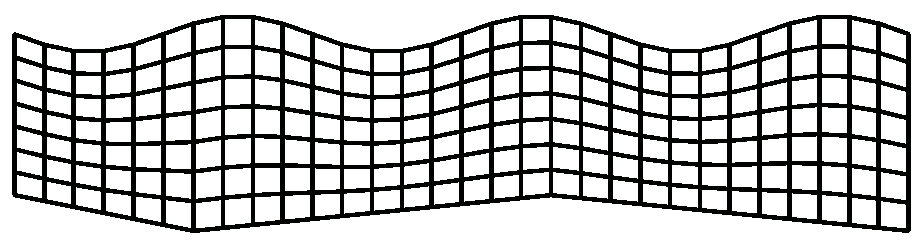
\includegraphics[width=8cm]{tube2.png}
\end{center}
\caption{Tube with 200 bilinear rectangles.
a) straight tube with 
two kinds of mesh refinement
b) sinusoidal and linear boundary mappings}
\label{pic3}
\end{figure}

\subsection*{Square with holes: \texttt{holes.grd}}

The subcell structure may be quite complicated. This is reflected by an
example of a square with a large number of square holes. Even at such a complicated
case almost the desired amount of elements may be created quite quickly.
The second case with 81 holes and 112000 elements was created in 
about a second an a normal PC.
\verbatiminput{examples/holes.grd}
%
\begin{figure}
\begin{center}

\includegraphics[width=5.5cm]{holes.png}
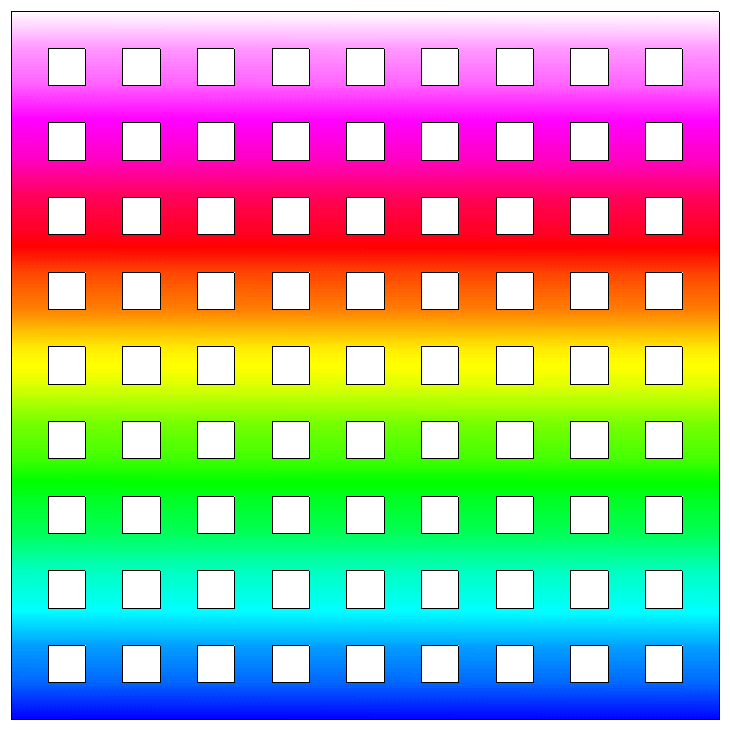
\includegraphics[width=5.5cm]{holes2.png}
\end{center}
\caption{Squares with holes: 
a) square with 16 square holes and 1040 elements,
b) square with 81 square holes and 112000 elements.}
\label{pic5}
\end{figure}


\subsection*{Cross: \texttt{cross.grd}}

To show that multiple mappings may be used at the same time
a more complicated case is given. Here two horizontal and two vertical lines
are mapped. The mesher has the nice property that the same file may be used
to created multiple meshes with different settings. The other mesh is now
the external mesh and it is divided to triangles.
\verbatiminput{examples/cross.grd}

\begin{figure}
\begin{center}
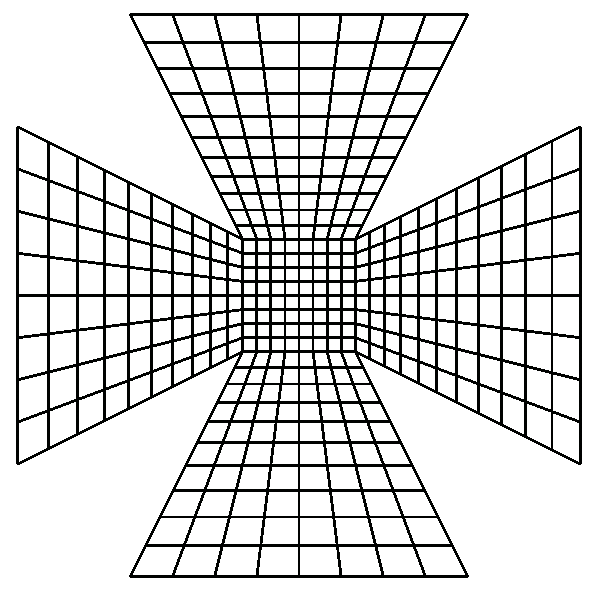
\includegraphics[width=5.5cm]{cross1.png}

\includegraphics[width=5.5cm]{cross2.png}
\end{center}
\caption{Cross with shape used to create 2 computational meshes:
      a) the internal mesh of 400 bilinear rectangles
      b) the external mesh of 800 linear triangles.}
\label{pic7}
\end{figure}

\subsection*{Hand-weight: \texttt{weight.grd}}

\verbatiminput{examples/weight.grd}
%
The extrusion requires that there are subcells also in the 
$z$-direction. In this case only one subcell is set.
\begin{verbatim}
Coordinate System = Cartesian 3D
Subcell Divisions = 3 3 1
\end{verbatim}

\noindent
In addition all information that is given for $x$ and $y$
must now also be given for $z$. For example, the 
subcell boundaries in the extruded direction must be given.
\begin{verbatim}
Subcell Limits 3 = 0.0 0.5
\end{verbatim}

\begin{figure}
\begin{center}

\includegraphics[width=8cm]{weight.png} 
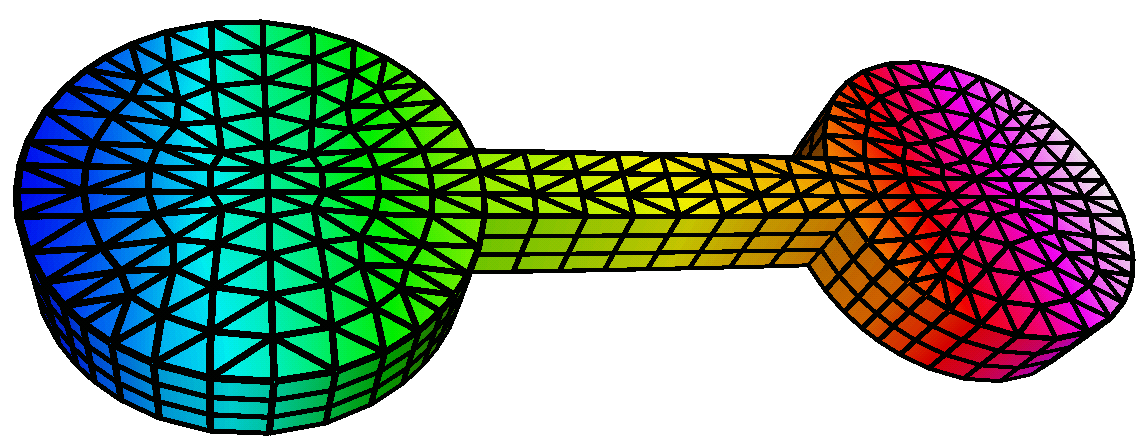
\includegraphics[width=8cm]{weight3.png}
\end{center}
\caption{Hand-weight consisting of two spheres and a joining tube
      a) 2D mesh with 1000 linear triangles
	b) extruded 3D mesh with 1200 prisms.}
\label{pic8}
\end{figure}



\section{3D examples}

\subsection*{Shell of waves: \texttt{waves.grd}}

The originally 2D mesh may be given a third dimension with the help of mapping.
In this example two sinusoidal mappings are used. They have a amplitude
with different sign and therefore there is a phase-shift of 180 degrees between the 
two opposing sides. 

\begin{figure}
\begin{center}
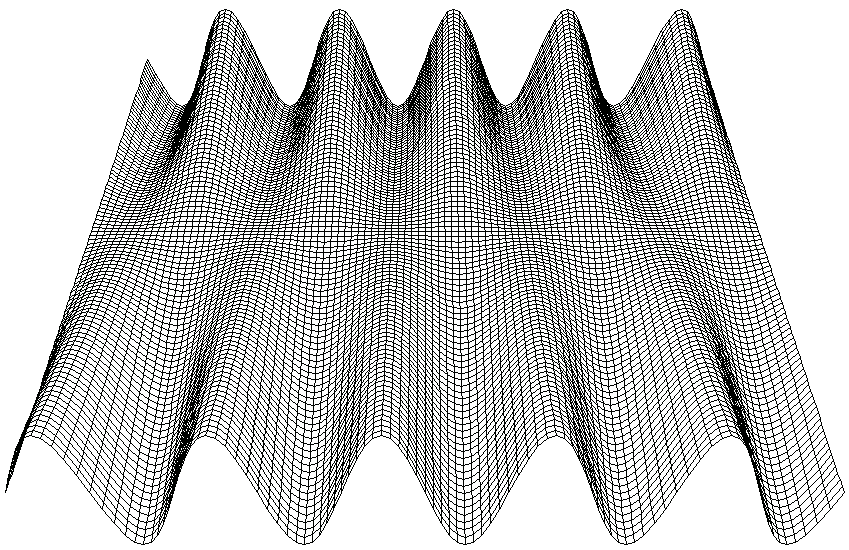
\includegraphics[width=7cm]{waves.png}
\end{center}
\caption{A shell with a wave pattern}
\label{pic9b}
\end{figure}

\verbatiminput{examples/waves.grd}


\subsection*{Shell consisting of two adjacent cones: \texttt{cones.grd}}

There are some cases where a mesh consisting of 2D elements 
may be used to model also 2D geometries. This is the case for
thin shells, for example. ElmerGrid does offer limited 
functionality for creating these. Only 
shells with rotational symmetry are possible to be created. 
Then the computational mesh is done for the $z$ and $\phi$ variables.
The missing radius must also be given.
After that $x=r \cos \phi$ and $y= r \sin \phi$.
Also limited possibilities to alter the radius as 
a function of positions is given. The same mappings may be used
as for 2D meshes in cartesian coordinates.

The examples shows a simple cylinder where a mapping is
used to create two cones. 

\begin{figure}
\begin{center}
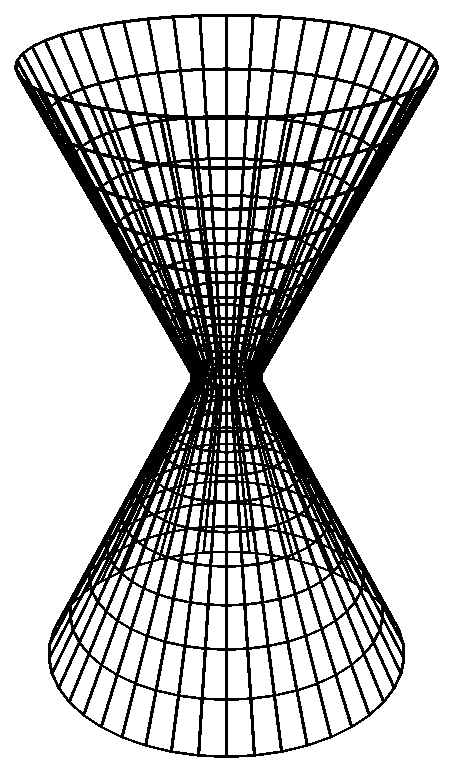
\includegraphics[width=6cm]{cones.png}
\end{center}
\caption{A 2D mesh mapped into two 3D cones}
\label{pic10}
\end{figure}

\verbatiminput{examples/cones.grd}


\subsection*{A rolled shell: \texttt{cones.grd}}

The mappings out of plane may also be used to create a simple roll.
Now the angles extends to 3600 degrees making 10
full rotations. The radius goes linearly from 1 to 101 and thus the
roll has a spiraling structure.

\begin{figure}
\begin{center}

\includegraphics[width=7cm]{roll.png}
\end{center}
\caption{A rolled shell with a spiraling structure}
\label{pic11}
\end{figure}

\verbatiminput{examples/roll.grd}


\subsection*{A hexagonal frame: \texttt{hexframe.grd}}

There is also a very special mapping for creating 
3D shell structures. The mapping is used to give an
angle for the shell. The angle is stepwise constant which makes
is possible to create polygonal 3D shells.  

\begin{figure}
\begin{center}
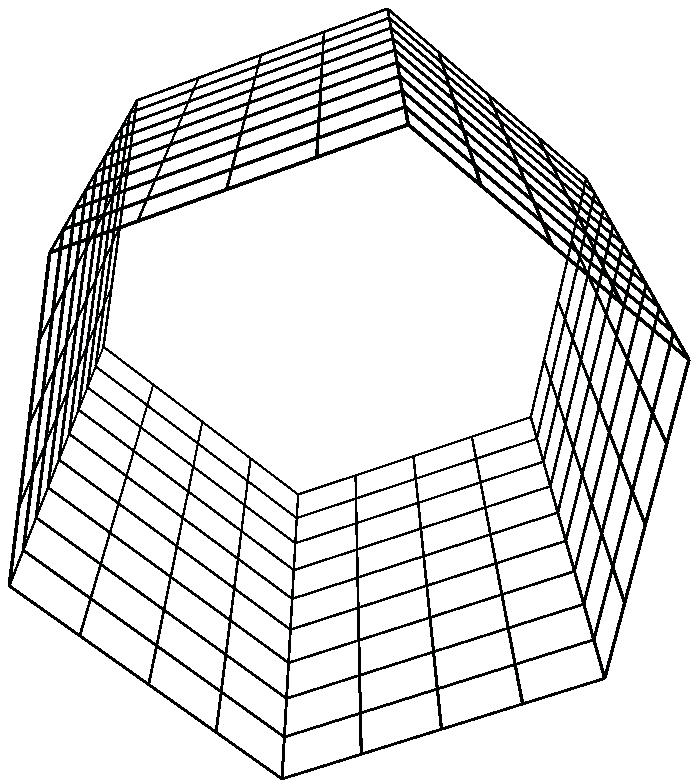
\includegraphics[width=7cm]{hexframe.png}
\end{center}
\caption{A hexagonal 3D frame made by mapping by angle}
%\label{pic11}
\end{figure}

\verbatiminput{examples/hexframe.grd}



\subsection*{Rotated step structure: \texttt{barrel.grd}}

\begin{figure}
\begin{center}
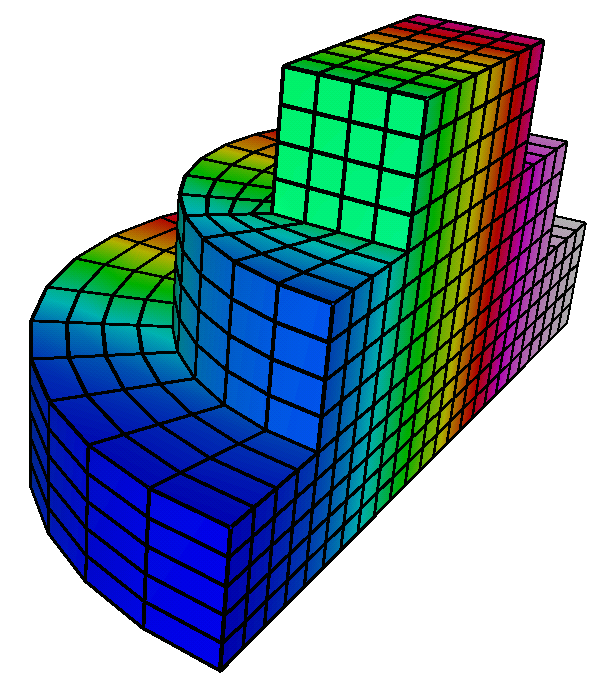
\includegraphics[width=8cm]{barrel.png}
\end{center}
\caption{Step structure rotated 180 degrees to create
      3D object with 1312 elements}
\label{pic9}
\end{figure}

\verbatiminput{examples/barrel.grd}


\subsection*{Extruded structure: \texttt{blocks.grd}}
The 2D structures may be extruded in the third dimension. 
Then the third dimension is added to the subcells
boundaries and to the mesh definitions.

The material
structure is always 2D. 
The given material structure may be 
extruded as is, or alternatively a selective extrusion for
different materials may be performed as is done in this example.
It is therefore possible to omit some materials, and to rename 
the extruded layer to some new material.

\begin{figure}
\begin{center}
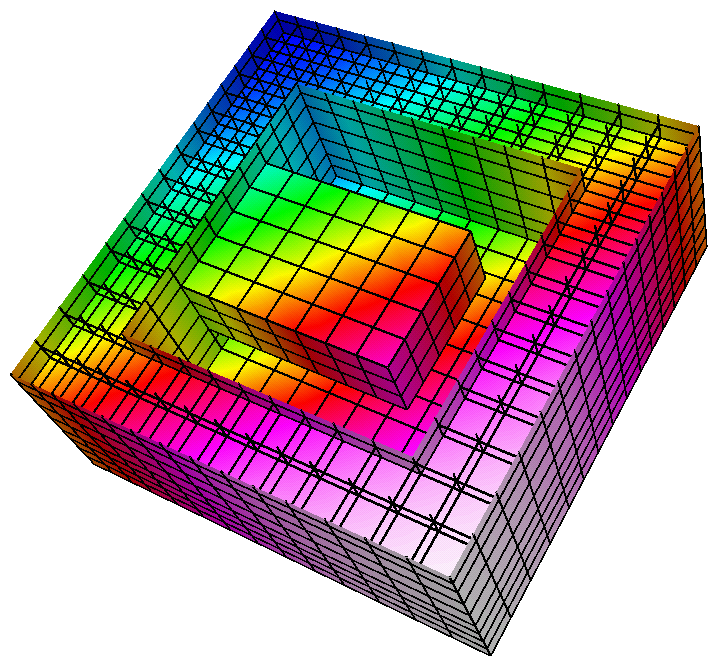
\includegraphics[width=8cm]{blocks.png}
\end{center}
\caption{Simple 3D structure created by selective extrusion. 
	The upper part has been removed for visualization purposes.}
\label{pic12}
\end{figure}

\verbatiminput{examples/blocks.grd}


\section{1D examples}

The ElmerGrid program was originally written for 2D mesh generation. 
However, it is also possible to make even more trivial one dimensional grids.
This is rarely needed as most FEM computations are at least two dimensional.

\subsection*{Line: \texttt{line.grd}}

The example of the 1D case is naturally a line segment -- there are no other kind of basic 1D structures.
It consists of two sections, the first one has a increasing mesh density to the right and the second one
has an even distribution of nodes.
\verbatiminput{examples/line.grd}

\begin{figure}
\begin{center}

\includegraphics[width=12cm]{line.png} 
\end{center}
\caption{A line segment where the element nodes are marked with polygons.
The mesh has 50 elements and thus 51 nodes.}
\label{pic8b}
\end{figure}


\graphicspath{{./}{tool/}}
\chapter{ElmerGrid mesh manipulation examples}

ElmerGrid may often be used as a grid manipulation
tool even though the computational mesh would 
originally have been made by some other mesh
generator. There are many basic 
operations, such as scaling or rotation, which do not 
require any special attention. Here we look at some more 
advanced things that may be performed an a mesh. 



\section{Mesh partitioning}

Nowadays the best performance from computers is obtained using
parallel solution techniques. In finite element method this
means that the mesh must be divide into separate domains 
that are solved by single processors. The domains should 
be chosen so that the extra work needed for the communications is
minimized. This procedure is called mesh partitioning. 
ElmerGrid offers two different techniques for this. 
The first one used Metis library and the second one divides the
mesh using simple ordering schemes. 

As an example we choose an L-shaped domain of bilinear elements.
The grid file for creating this one is given below.
\verbatiminput{tool/angle.grd}

The partitioning may be invoked using command line arguments, or
as here using command file. Below is the command file
for using the simple partitioning scheme to partition the
mesh into $2 \times 2$ domains. 
%
\verbatiminput{tool/part.eg}
%
In the start of the command file the user defines the input and 
output formats and filenames. The only additional command is the 
last line that defines how the mesh is partitioned.
Another choice is to use Metis which is invoked with the line
\begin{verbatim}
Metis = 4
\end{verbatim}
The resulting partitionings are shown in Figure~\ref{pic50}. In this case
the partitionings are almost equally good. In very simple
cases the simple geometrical algorithm may give better results
but in general cases Metis should be favored.
%
\begin{figure}
\begin{center}

\includegraphics[width=7cm]{part.png}

\includegraphics[width=7cm]{metis.png}
\end{center}
\caption{A simple mesh partitioned with a simple geometrical scheme and 
Metis library.}
\label{pic50}
\end{figure}


\section{Boundary layer creation}

In nature there are often sharp changes in the physical 
behavior which may be seen in forms of boundary layers.
Particularly in the area of fluid dynamics boundary layers
are often of special interest. 
A physical boundary layer requires
a suitable computational mesh if one 
wants to model the physical phenomena accurately. 
Equally tight mesh is not usually needed elsewhere and thus
an optimal solution is a proper boundary layer mesh.
Ideally the mesh is such that the elements are small only in the 
direction of the gradient. 

ElmerGrid includes a simple 2D capability for creating boundary layer
meshes. There the user may choose the boundary conditions of interest 
and extrude them in the direction of the normal to create a structured 
mesh just on the boundary. The new mesh may also be fitted into the 
size of the original mesh using a simple Jacobian smoother which
tries to maintain the geometrical shape of the mesh. 
Often this is not so easy and therefore the methodology may create
some complications on the corner nodes, for example.

The example case chosen is the same one as for the 
partitioning example except the number of plane elements is reduced to
300 to make the boundary layer more visible.
In the geometry there is only one boundary and therefore 
only one boundary layer is also created. There can however be several
boundary layers at a time. In the intersections of different boundary
layers one should however notice that the number of new elements should be
the same. The resulting mesh is shown in Figure~\ref{pic51}.
%
\verbatiminput{tool/layer.eg}

\begin{figure}
\begin{center}
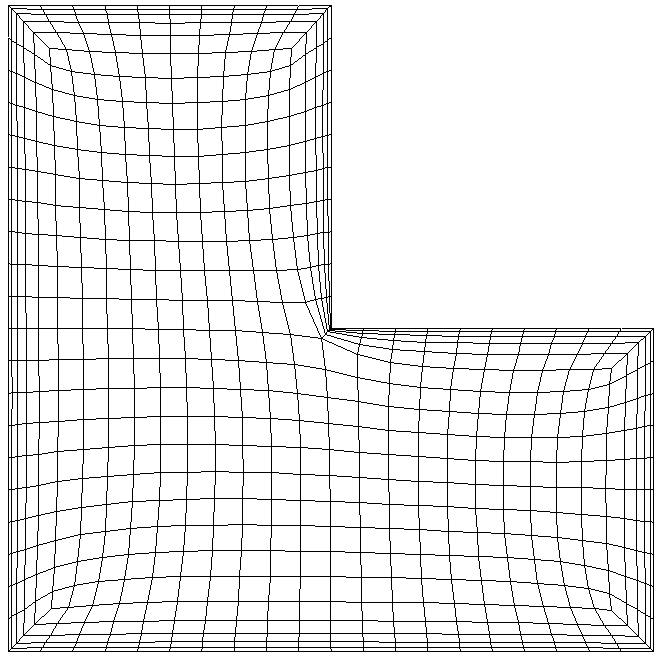
\includegraphics[width=7cm]{layer.png}
\end{center}
\caption{A simple boundary layer created on an angle mesh}
\label{pic51}
\end{figure}

\section{Mesh extrusion}

ElmerGrid enables that any mesh on a plane may be extruded in the 
third dimension by given the specifications on how to extrude.
For example the command file below may be used to extrude the mesh 
created in the first example in the third dimension. The result is a unit 
cube with 1000 trilinear elements.
%
\verbatiminput{tool/rect2cube.eg}
%
\begin{figure}[bh]
\begin{center}
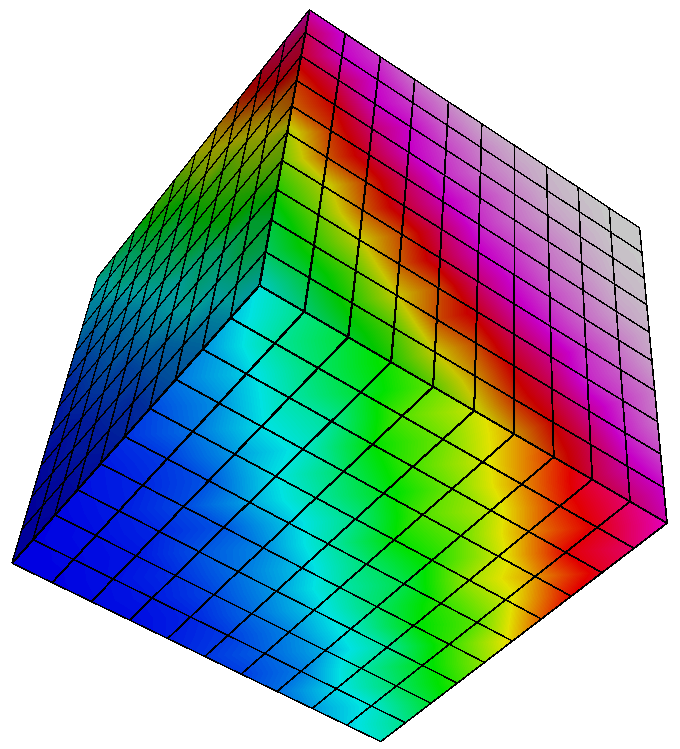
\includegraphics[width=7cm]{cube.png}
\end{center}
\caption{A simple cube created by the extrusion of a unit square}
\label{pic52}
\end{figure}


\graphicspath{{./}{import/}}
\chapter{ElmerGrid Interface Examples}

ElmerGrid understands a number of different mesh formats which 
enables the import from meshes created by other mesh generators into
the Elmer solution cycle. Supported formats includes those by Ansys (separate macro), 
Abaqus, Gambit (FDNET), Comsol Multiphysics, Fieldview, Triangle, 
Medit, Gsmh, and GiD.

\section{Ansys mesh to Elmer}

The APDL macros and the following documentation have been written
by {\em Antti Pursula} (email: Antti.Pursula@csc.fi). He will 
answer any further questions related to the macros.

Two APDL (Ansys parametric design language) macros has been created
which allow writing geometry data in ASCII format out of Ansys. The
macros can be activated from Ansys GUI using custom added buttons in
the Ansys Toolbar. The ASCII format files can further be converted in
the Elmer format by using ElmerGrid.

The information written out by the macros consists of four files that
are named \texttt{ExportMesh.*} (\texttt{* = header, node, elem}, or
\texttt{boundary}). The files include all the information Elmer needs for using
the mesh ie., besides the obvious node and element definitions, also
information about the boundary nodes. 

%Detailed information of the file
%formats is found here (in Finnish), but this information is not needed
%in any way when using Ansys to Elmer interface.

In Ansys, the geometry model is often created combining several
elementary geometries. This means that the model usually includes
boundaries, that have no physical meaning. These do not disturb the
analysis neither in Ansys nor in Elmer, but they can make the
definition of boundary conditions quite cumbersome in
Elmer. Therefore, there are two possible macros for exporting data
from Ansys: ELMER\_AU and ELMER\_CH. The first writes all the boundaries
of the model automatically while the second asks the user to
graphically pick the boundaries that have physical meaning. It is
worthwhile to notice that Elmer does not necessarily need boundary
information for all the physical boundaries, but only those on which a
boundary condition is to be applied.

To use Ansys to Elmer interface you need to download two macro files
and an Ansys start-up file and copy them into your working
directory. After the files have been copied, start Ansys and the
buttons ELMER\_AU and ELMER\_CH appear in the Toolbar. The conversion of
the resulting ASCII files into Elmer format is done by the ElmerGrid
program. The files as well as ElmerGrid can be downloaded from the
Elmer download page.

%ElmerGrid is controlled through command line arguments. 
%
%The syntax is
%ElmerGrid input\_format output\_format filename [options]. The input and
%output formats are numbers. 
%
In ElmerGrid the Ansys input format is 4 and output
format can be Elmer mesh format (3) or ElmerPost format (2). So,
creating Elmer meshes from Ansys input is done with the command:
\texttt{ElmerGrid 4 3 ExportMesh}. There are also many command-line 
options available. The
most important ones in this case are:
%
\begin{itemize}
  \item \texttt{-o name} for saving output with the name specified.  
  \item \texttt{-order $c_x$ $c_y$ $c_z$} for reordering nodes and elements using $c_1x+c_2y +c_3z$.  
  \item \texttt{-scale $c_x$ $c_y$ $c_z$} for scaling the mesh using the constant to multiply
the coordinate values.
  \item \texttt{-merge epsilon} for merging nodes that are at most distance epsilon apart.
\end{itemize}

The \texttt{-merge} option is important in a case where Ansys creates multiple
nodes on a boundary of two elementary geometries. These nodes are
often noticed only when Elmer is not able to use a mesh created from
Ansys. In such a case, use \texttt{-merge} option with a suitable value 
for the node separation.

\begin{figure}
\begin{center}
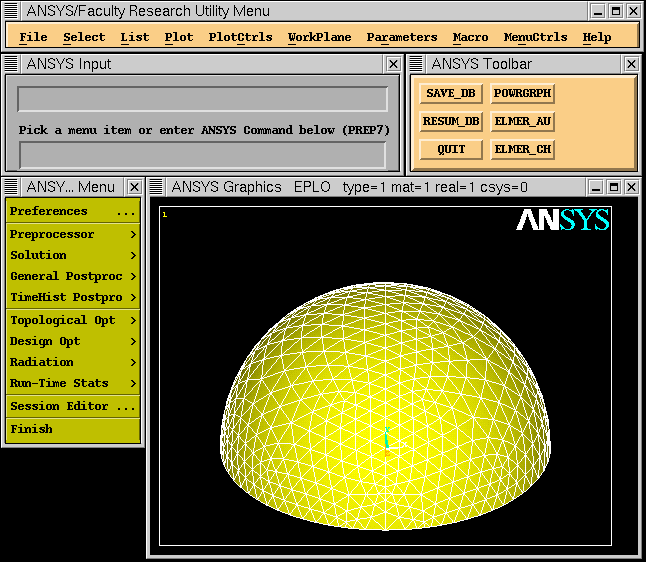
\includegraphics[height=5cm]{ansys2elmer-a}
\hspace{10mm}
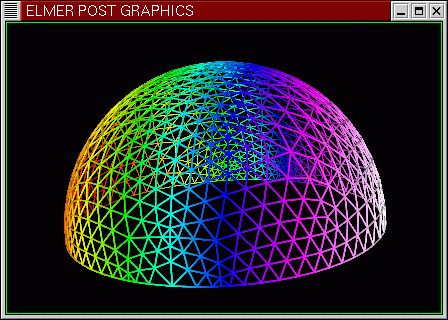
\includegraphics[height=5cm]{ansys2elmer-b}
\end{center}
\caption{Pictures of the same mesh in Ansys desktop and in ElmerPost window.}
%\label{pic5}
\end{figure}


\section{Comsol Multiphysics to Elmer}

Comsol Multiphysics is a widely used finite element tool with highly 
automated mesh generation. Previously the software was known as Femlab. 
In the older versions of Comsol Multiphysics/Femlab there 
wasn't any export format that would have included the boundary definitions. 
However, since version 3.2 of Comsol Multiphysics there 
is a suitable export format that may be directly used to export meshes in Elmer 
-- the mphtxt format. 
The ElmerGrid program 
understands a sufficient subset of the commands in mphtxt-file of 
Comsol multiphysics. 

%There are two different strategies depending whether one uses the old or new
%version. 
%The ElmerGrid utility tries first to apply the Comsol Multiphysics strategy and then
%uses the older Matlab version. 

%\subsection{Comsol Multiphysics with pmhtxt-export}

The procedure for importing meshes to Elmer is
\begin{itemize}
  \item In Comsol Multiphysics choose \\
   \texttt{File -> Export -> Mesh to File}
   \item Select the export format \\ \texttt{``COMSOL Multiphysics text file'' (mphtxt)}
   \item Give the mesh a file name, e.g. \texttt{mymesh} and you obtain the 
    file \texttt{mymesh.mphtxt}
  \item Call then ElmerGrid with the following command line options to obtain E
ElmerSolver mesh file format \\
    \texttt{ElmerGrid 9 2 mymesh.mphtxt}
  \item And with the following options to obtain ElmerPost result format \\
    \texttt{ElmerGrid 9 3 mymesh.mphtxt}
\end{itemize}
%As a result you get a directory \texttt{mymesh} which may be used in Elmer 
%computations. 
%The utility should be backward compatible for some time.


%\subsection{Femlab version bundled with Matlab}

%The original version of Femlab was bundled with 
%Matlab and therefore a natural approach to export results from Femlab was 
%to use a .m script that provided all the necessary information. 
%The mesh export strategy is applicable for 2D and 3D meshes consisting
%of triangles, and for 3D tetrahedral meshes. It is not possible to
%combine volume and surface meshes unless the surface is part of the
%volume mesh. The needed export utility for Femlab/Matlab is obtained from
%the Elmer download page

%The export is performed in following steps:
%\begin{enumerate}
%\item When you have created a mesh in Femlab choose \texttt{Export to
%Workspace} and thereafter \texttt{Mesh}. The suggested name is \texttt{mesh}, but that
%may be changed.  
%
%\item Then go to Matlab and run the provided 
%command-file \texttt{savemesh.m}. The only parameter is the name of the mesh
%data, e.g. \texttt{savemesh(mesh)}. This command then creates files \\
%FemlabMesh.header: information of vector sizes  \\
%FemlabMesh.node: node coordinates  \\
%FemlabMesh.elem: element topologies  \\
%FemlabMesh.boundary: boundary side definitions  
%
%\item To transform the mesh for a format known by
%Elmer use ElmerGrid. The flag for Femlab export format is 9. Use the
%following commands:  \\
%\texttt{ElmerGrid 9 2 meshname}: for making mesh files
%usable by ElmerFront and ElmerSolver  \\ 
%\texttt{ElmerGrid 9 3 meshname}: For viewing the mesh with ElmerPost  
%You may also use many ElmerGrid
%options, such as \texttt{-order real[3]} 
%where the vector orders the nodes to
%decrease the matrix bandwidth, e.g. \texttt{ElmerGrid 9 2 meshname -out outname
%-order 1.0 2.0 3.0}
%\end{enumerate}

\begin{figure}
\begin{center}
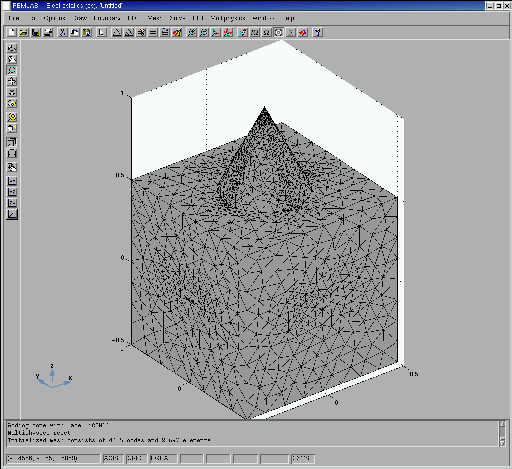
\includegraphics[height=5cm]{femlab2elmer-a}
\hspace{10mm}
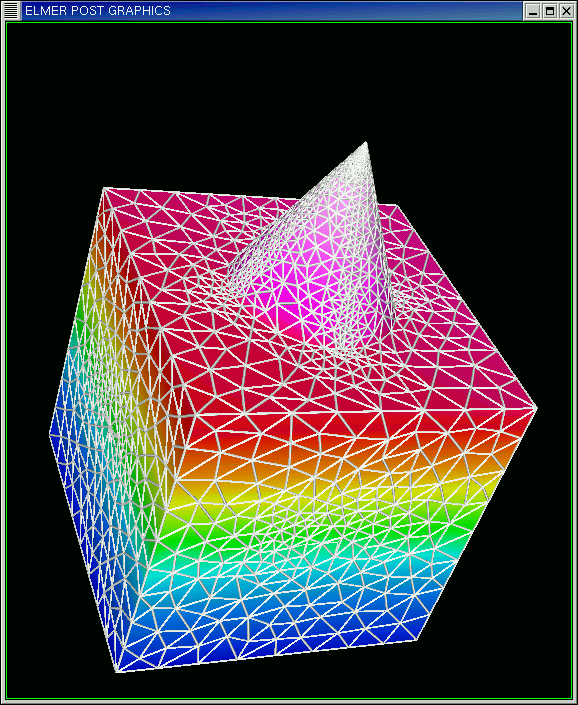
\includegraphics[height=5cm]{femlab2elmer-b}
\end{center}
\caption{Pictures of the same mesh in Femlab desktop and in ElmerPost window.}
%\label{pic5}
\end{figure}


\section{Triangle mesh to Elmer}

Triangle is a two-dimensional quality mesh generator and Delaunay triangulator.
written by Jonathan Richard Shewchuk
in University of California at Berkeley (email: jrs@cs.berkeley.edu).

The format written by Triangle is very similar to that one needed by Elmer. 
The only problem is to find the boundaries defined by the nodes known
to lie on the boundary. The current implementation of the algorithm may
result to problems at the corners. Also the functionality hasn't been tested for
cases with several materials or several boundaries.

Assuming we have a triangle input file name \texttt{tri.poly}. This may be meshed 
with second order triangles having all corners above 32.0 degrees and 
area below 0.001 with the command
\begin{verbatim}
triangle -pq32.0 -a.0001 -o2 tri
\end{verbatim}
\noindent This creates files \texttt{tri.i.ele} and \texttt{tri.i.node}
 (i=$1,2,\ldots$),
which may be used to create the Elmer model.

The Triangle format corresponds to input mode 11 at ElmerGrid. Therefore
the mesh for ElmerSolver is created with command
\begin{verbatim}
ElmerGrid 11 2 tri.1
\end{verbatim}
\noindent
which results to a computational mesh being saved at ElmerSolver format in
subdirectory \texttt{tri}.

\begin{figure}
\begin{center}

\includegraphics[height=5cm]{triangle2elmer}
\end{center}
\caption{Picture of the Triangle example case in ElmerPost.}
%\label{pic5}
\end{figure}





%%%%%%%%%%%%%%%%%%%%%%%%%%%%%%%%%%%%%%%%%%%%%%%%%%%%%%%%%%%%
% Appendices 

%\appendix

%%%%%%%%%%%%%%%%%%%%%%%%%%%%%%%%%%%%%%%%%%%%%%%%%%%%%%%%%%%%

% Include the index
\phantomsection
\addcontentsline{toc}{chapter}{Index}
\printindex


\end{document}

%%%%%%%%%%%%%%%%%%%%%%%%%%%%%%%%%%%%%%%%%%%%%%%%%%%%%%%%%%%%


